% ------------------------------------------------------------------------------
% Este fichero es parte de la plantilla LaTeX para la realización de Proyectos
% Final de Grado, protegido bajo los términos de la licencia GFDL.
% Para más información, la licencia completa viene incluida en el
% fichero fdl-1.3.tex

% Copyright (C) 2012 SPI-FM. Universidad de Cádiz
% ------------------------------------------------------------------------------

A continuación se detallan las instrucciones de uso de la aplicación
EasyData/Django, las cuales deberá seguir para un correcto funcionamiento de la
aplicación.

% Las instrucciones de uso del sistema se detallan a continuación.

\section{Introducción}

El presente capítulo es un manual de usuario, el cual le permitirá tener los
conocimientos necesarios para poder utilizar la aplicación EasyData/Django. Esta
aplicación le permitirá realizar un mapeo entre cada uno de los modelos de su
proyecto Django donde instale la aplicación, y diferentes ontologías existentes
en la web, para posteriormente realizar la publicación de sus datos en función
al mapeo que ha realizado con dichas ontologías, de tal forma que el contenido
de su aplicación, sea perfectamente entendible por cualquier entidad que acceda.

Haciendo uso de las ontologías anteriormente citadas, al tratarse de espacios de
nombres establecidos, estará marcando su contenido web de forma que los datos
que aquí figuren sean mucho más comprensibles, ya que esta dotando a los datos
que publica de un mayor contenido semántico.

Siga este manual, una vez haya concluido con la instalación de la aplicación
EasyData/Django, tal y como se detalla en el apartado \ref{chap:maninsexp}, de
la presente memoria.

% Resumen de los principales objetivos, ámbito y alcance del software desarrollado.

\section{Características}
\label{sec:caracteristicas}
Las características o funcionalidades principales que le ofrece la aplicación
EasyData/Django, son las que se especifican a continuación:
\begin{itemize}
    \item Captación de los modelos y fields que componen su proyecto Django.
    \item Carga de namespaces u ontologías.
    \item Configuración de la privacidad de los datos.
    \item Mapeo de modelos y fields de su proyecto con las entidades y
          propiedades de las distintas ontologías.
    \item Publicación de datos en diferentes formatos.
    \item Generación de fichero D2Rq con la configuración realizada en la
          aplicación.
    \item Generación de gráfico con la configuración del mapeo.
\end{itemize}

% Recopilación de las principales funcionalidades del sistema.

\section{Requisitos previos}

Los requisitos previos que debe cumplir la máquina donde vaya a instalarse la
aplicación EasyData/Django son los siguientes:
\begin{itemize}
    \item Sistema operativo con soporte para la ejecución de código python.
    \item Versión de python 2.6 o 2.7.
    \item Versión de Django igual o superior a la 1.4.
    \item Paquete rdflib de python en su versión 4.0.1.
\end{itemize}

% Requisitos hardware y software para el correcto uso del sistema.

\section{Utilización}

A continuación, se va a explicar como realizar cada una de las funcionalidades
comentadas en el apartado \ref{sec:caracteristicas}. La explicación de las
mismas, se realiza en el mismo orden en que deberán de llevarse a cabo para que
todo funcione correctamente.

\subsection{Captación de modelos y fields}

La captación de modelos y fields por introspección de su proyecto Django es
bastante sencilla. Este procedimiento se lleva a cabo desde el manage.py de su
proyecto Django, ya que la aplicación EasyData/Django añade una nueva opción al
manage.py, que le permitirá realizar este procedimiento con toda facilidad.

Para ello únicamente deberá de dirigirse al directorio de su proyecto Django
donde se encuentra el fichero manage.py, y desde una terminal de escritorio,
deberá ejecutar el siguiente comando:

\begin{lstlisting}[frame=L, language=bash, basicstyle=\footnotesize]
$> python manage.py loadmodels
\end{lstlisting}

Una vez el proceso de carga de los modelos y fields haya concluido, se le
informará mediante un mensaje. En la figura \ref{fig:loadmodels} puede ver el
resultado de como sería el proceso de captación.

\begin{figure}[H]
    \begin{center}
        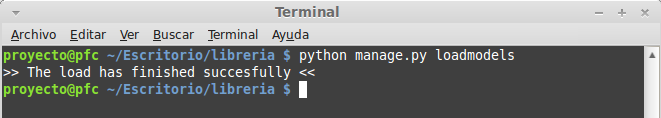
\includegraphics[width=1\textwidth]{manual_usuario/loadmodels.png}
    \end{center}
    \caption{Resultado de captación de modelos y fields}
    \label{fig:loadmodels}
\end{figure}

\subsection{Carga de namespaces}

El siguiente paso imprescindible para poder realizar el mapeo de sus modelos con
las ontologías, es tener alguna cargada en la aplicación. La carga de ontologías
o namespaces en la aplicación, se hace desde dentro de la aplicación, en el
apartado llamado Namespace.

Cuando acceda a este apartado, le aparecerá una lista con todos los namespaces
disponibles (Figura \ref{fig:lista_namespace}) para ser usados (inicialmente la
lista estará vacía). Desde este apartado, podrá tanto añadir nuevos namespaces
(Figura \ref{fig:nuevo_namespace}), como editarlos/actualizarlos (Figura
\ref{fig:editar_namespace}), o incluso eliminarlos\footnote{Tenga especial
cuidado a la hora de borrar los namespaces, ya que perderá también la
configuración que tenga entre sus modelos y el namespace. A la hora de borrar un
determinado namespace, se advertirá al usuario de que esté seguro de realizar
esta acción.}.

\newpage

\begin{figure}[H]
    \begin{center}
        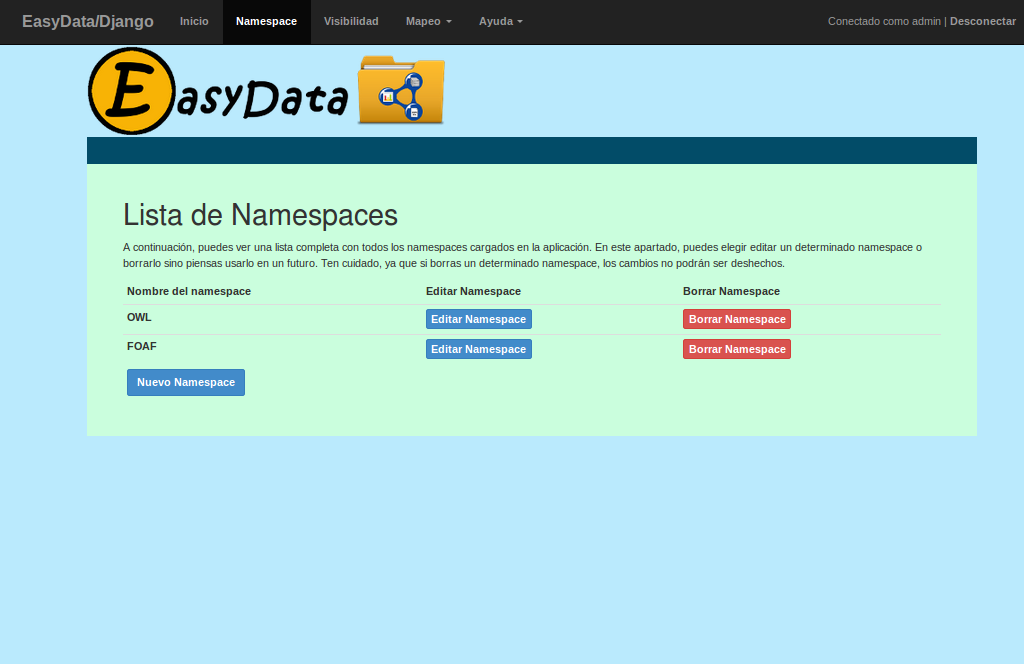
\includegraphics[width=0.9\textwidth]{manual_usuario/lista_namespace.png}
    \end{center}
    \caption{Listado de namespaces cargados en la aplicación}
    \label{fig:lista_namespace}
\end{figure}

\begin{figure}[H]
    \begin{center}
        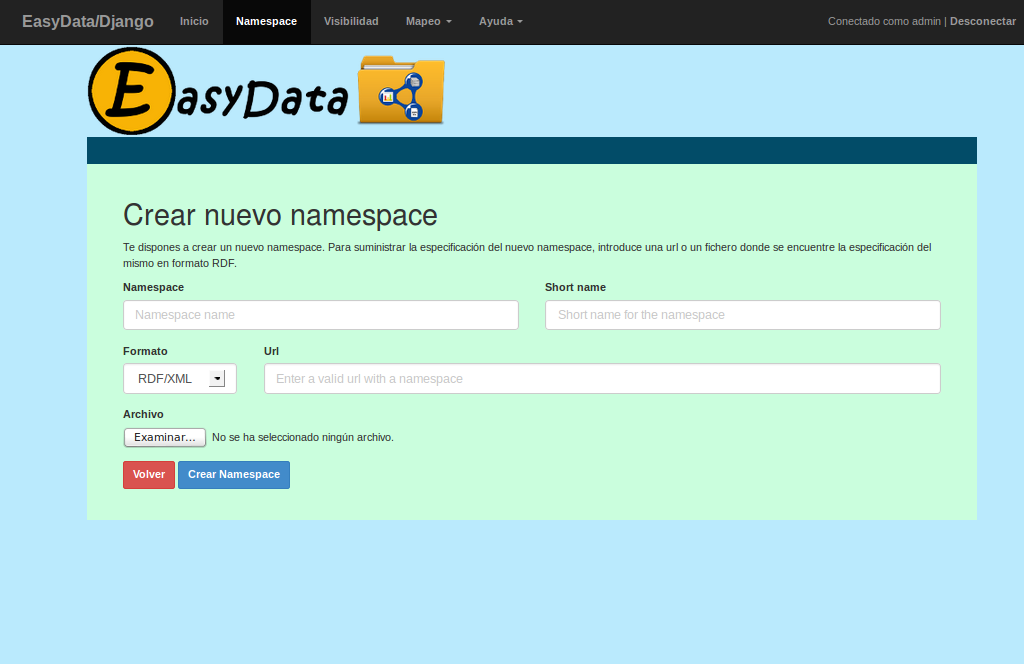
\includegraphics[width=0.9\textwidth]{manual_usuario/nuevo_namespace.png}
    \end{center}
    \caption{Formulario de creación de un nuevo namespace}
    \label{fig:nuevo_namespace}
\end{figure}

\begin{figure}[H]
    \begin{center}
        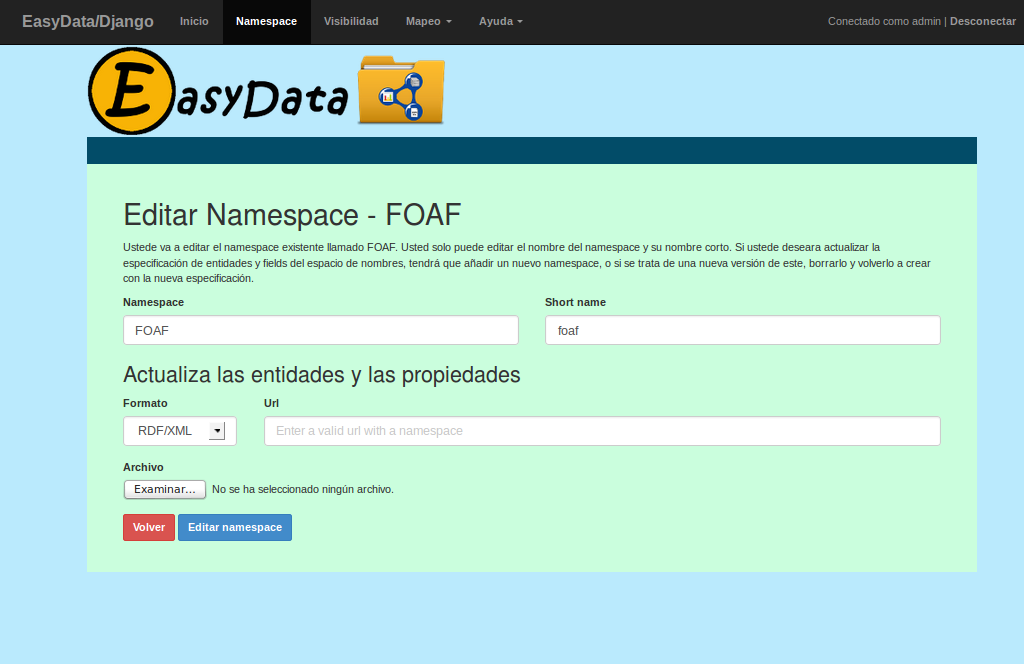
\includegraphics[width=0.9\textwidth]{manual_usuario/editar_namespace.png}
    \end{center}
    \caption{Pantalla de edición de un namespace existente}
    \label{fig:editar_namespace}
\end{figure}

Para cargar un nuevo namespace, pulse sobre el botón azul de
\textit{Nuevo Namespace}, y le aparecerá un formulario donde se le solicitará
la siguiente información:
\begin{itemize}
    \item \textbf{Namespace:} esto es un nombre identificativo que recibirá el
        namespace, el cual no influye en el mapeo. Este dato es único y no puede
        repetirse. Tiene como máximo 40 caracteres.
    \item \textbf{Short name:} este dato hace referencia a un nombre corto que
        represente el namespace, el cual se utilizará a la hora de generar tanto
        el RDF como RDFa, etc... Este dato es único y no puede repetirse con
        otros ya existentes. Tiene como máximo 15 caracteres.
    \item \textbf{Formato:} es el formato del fichero que se suministra con la
        especificación de la ontología. Actualmente están disponibles los
        formatos RDF/XML y RDF/Ntriples.
    \item \textbf{Url:} Es una url donde se encuentra el fichero con la
        especificación del namespace. Este dato no es obligatorio y solo debe
        suministrarse la url o el archivo.
    \item \textbf{Archivo:} Es un fichero donde se encuentra la especificación
        del namespace. Este dato no es obligatorio y solo debe suministrarse la
        url o el archivo.
\end{itemize}

Una vez introducidos los datos, pulse en \textit{Crear Namespace}, para cargar
el mismo en el sistema. Este proceso puede tardar un poco, en función del tamaño
del namespace, ya que se debe de leer toda la especificación y cargarla en la
base de datos.

Una vez se haya creado el namespace, se le redirigirá a la vista principal de
namespaces, y podrá observar que aparece en la lista el nuevo que acaba de
crear. Si por el contrario hubo algún error, se le informará y deberá de
corregir el formulario.

A la hora de editar/actualizar un namespace, le aparecerá un formulario similar
al de creación de un nuevo namespace, donde los campos nombre y short name,
aparecerán rellenos con los datos del namespace, de tal forma que pueda editar
los mismos. Por otro lado, también encontrará los apartados de formato, url y
archivo, donde para este caso, la utilidad de los mismos difiere un poco al del
caso anterior, ya que esta vez se cargará la especificación de las entidades y
propiedades del namespace, para añadir nuevas entidades o propiedades nuevas que
pudiesen haber sido incluidas posteriormente en la especificación, o para
actualizar las relaciones existentes entre entidades y propiedades del
namespace, con el resto de entidades y propiedades de otros namespaces
existentes en la aplicación, que no existiesen anteriormente.

Tanto a la hora de cargar un nuevo namespace como de actualizar uno existente,
esto se hará como bien se puede apreciar en el formulario, haciendo uso de
ficheros en formato rdf. Para que la aplicación pueda reconocer tanto las
entidades como las propiedades y las relaciones entre los mismos, estos deben de
estar especificados haciendo uso de las siguientes etiquetas defindas en los
namespaces \href{http://www.w3.org/TR/rdf-schema/}{RDFS} y
\href{http://www.w3.org/TR/owl-ref/}{OWL}:
\begin{itemize}
    \item Para la identificación de clases:
    \begin{itemize}
        \item \textbf{rdfs:Class}.
        \item \textbf{owl:Class}.
    \end{itemize}
    \item Para la identificación de propiedades:
    \begin{itemize}
        \item \textbf{rdf:Property}.
        \item \textbf{owl:ObjectProperty}.
        \item \textbf{owl:DatatypeProperty}.
        \item \textbf{owl:AnnotationProperty}.
    \end{itemize}
    \item Para la obtención de características de las clases y propiedades:
    \begin{itemize}
        \item \textbf{rdfs:comment}: para captar una descripción de la entidad o
            propiedad.
        \item \textbf{rdfs:label}: para captar la etiqueta de la entidad o
            propiedad.
        \item \textbf{rdfs:domain}: indica a qué entidades pertenece una
            determinada propiedad.
        \item \textbf{rdfs:range}: indica con qué entidades se relaciona una
            determinada propiedad.
        \item \textbf{rdfs:subClassOf}: indica de qué entidad es hija una
            determinada entidad.
    \end{itemize}
\end{itemize}

\subsection{Configuración de la privacidad}

Un punto muy importante a la hora de exportar nuestros datos, es decidir qué
datos queremos que se publiquen y qué otros no, ya que en muchos casos, nos será
interesante evitar que ciertos datos puedan ser accedidos por terceras personas,
porque se traten de datos sensibles, como contraseñas, números de cuentas
bancarias, etc... o sencillamente porque no deseemos que estos puedan verse.

La aplicación le permite la posibilidad de decidir qué datos se ocultaran a los
usuarios a la hora de publicar los mismos. Esto se hará en el apartado de
\textit{Visibilidad} (Figura \ref{fig:configura_visibilidad}). En este apartado,
le aparecerá un listado con cada una de las aplicaciones instaladas en su
proyecto Django, y pulsando en configurar visibilidad de una determinada
aplicación, se le mostrará una nueva pantalla (Figura
\ref{fig:configura_visibilidad_2}) con una pestaña por cada uno de los modelos
que contiene la aplicación.

\begin{figure}[H]
    \begin{center}
        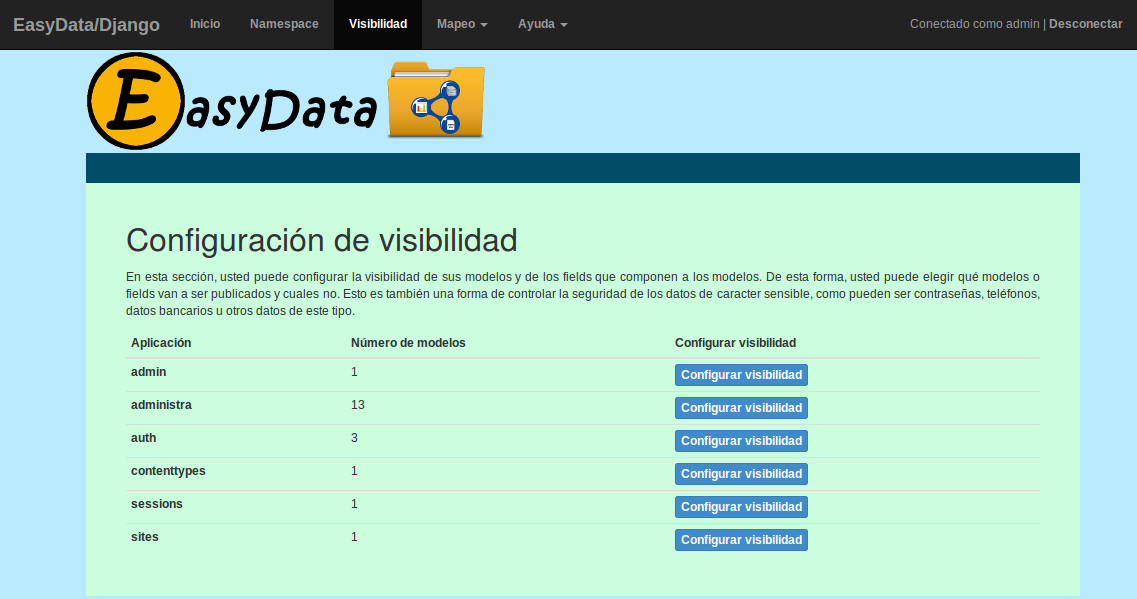
\includegraphics[width=0.95\textwidth]{manual_usuario/configura_visibilidad.png}
    \end{center}
    \caption{Pantalla de configuración de la privacidad - Aplicaciones}
    \label{fig:configura_visibilidad}
\end{figure}

En cada una de las pestañas de los modelos, podrá elegir si este modelo es
visible o privado completamente al exterior, o definirlo por fields en concreto,
indicando la visibilidad de los mismos.

Por defecto, para prevenir que inicialmente algún dato sea publicado por error,
todos los modelos están marcados como privados, de tal forma que será tarea del
usuario decidir cuáles de ellos se harán visibles.

\newpage

\begin{figure}[H]
    \begin{center}
        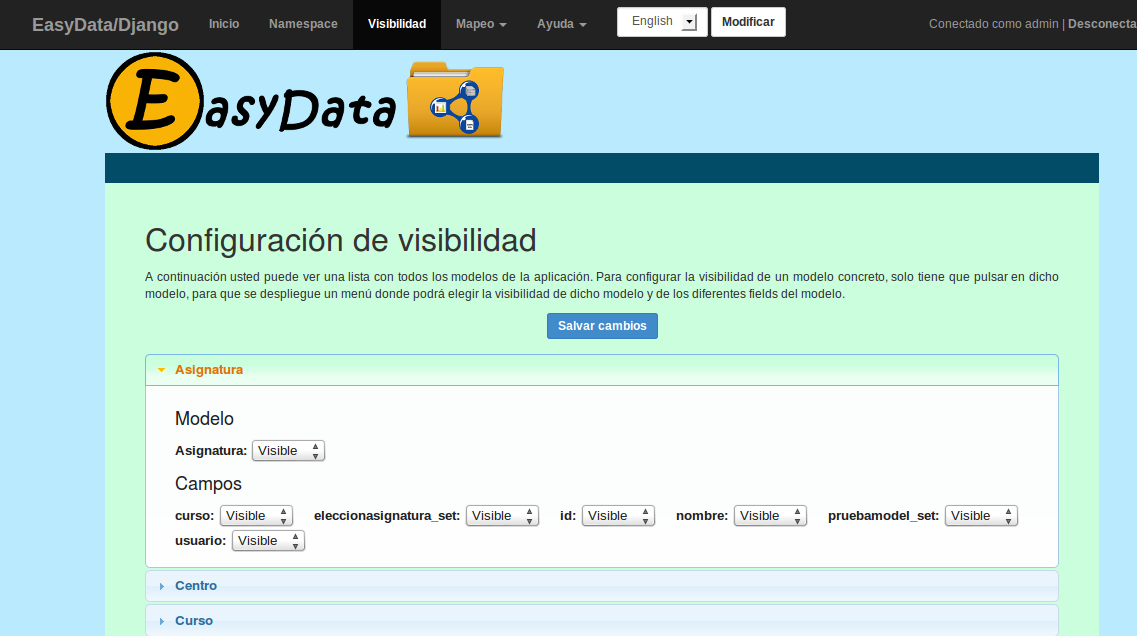
\includegraphics[width=0.95\textwidth]{manual_usuario/configura_visibilidad_2.png}
    \end{center}
    \caption{Pantalla de configuración de la privacidad - Modelos}
    \label{fig:configura_visibilidad_2}
\end{figure}

\subsection{Mapeo de modelos y fields}

El siguiente y último paso antes de la publicación de los datos, es indicarle a
la aplicación EasyData/Django, con qué entidades y propiedades de los distintos
namespaces van a estar relacionados nuestros modelos. Este paso se conoce como
el \textit{Mapeo de los datos}, y por consiguiente se llevará a cabo en el
apartado de la aplicación de \textit{Mapeo}.

Si accedemos a este apartado, nos aparecerá una lista desplegable (Figura
\ref{fig:mapea_modelos}). Cada uno de los elementos de la lista, representan a
cada una de las aplicaciones de nuestro proyecto. Si seleccionamos una de ellas,
para que se expanda dicho elemento, nos aparecerá cada uno de los modelos que
componen a dicha aplicación con dos elementos select. En esta parte realizaremos
el mapeo de los modelos, donde en el primero de los selects, seleccionaremos el
namespace que queremos utilizar de los que tenemos cargados en la aplicación, y
el siguiente select se cargará con las distintas entidades que componen al
namespace. De esta forma deberemos de mapear cada uno de los modelos que nos
interesen (no es necesario realizar el mapeo de todos, solo aquellos que nos
vaya a interesar publicar). Una vez realizado el mapeo de los modelos,
pulsaremos sobre el botón de \textit{Salvar cambios}.

\newpage

\begin{figure}[H]
    \begin{center}
        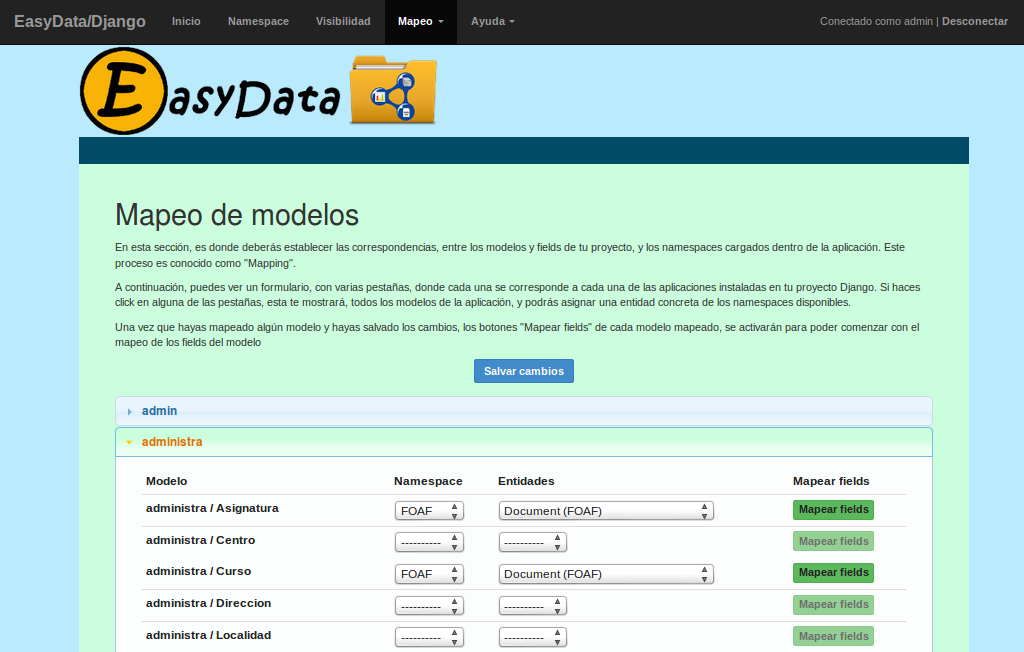
\includegraphics[width=1\textwidth]{manual_usuario/mapea_modelos.png}
    \end{center}
    \caption{Pantalla de mapeo de los modelos}
    \label{fig:mapea_modelos}
\end{figure}

Una vez hemos realizado el mapeo de los modelos y hemos salvado los cambios, se
activará el botón verde posicionado a la derecha de cada modelo que hemos
realizado su mapeo. Esto significa que podemos pasar ahora a realizar el mapeo
de los fields de dichos modelos, pulsando en dicho botón.

Cuando pulsemos sobre dicho botón, se nos llevará a un apartado parecido al
anterior, donde aparecerán por separado los atributos y relaciones del modelo
(Figura \ref{fig:mapea_fields}). Al igual que en el caso anterior, cada uno
dispondrá de dos selects, uno para elegir el namespace, y otro para elegir la
propiedad con la que deseamos mapear el field. Por defecto, aparece seleccionada
la entidad del namespace con que hemos mapeado el modelo, pero se puede
modificar para utilizar otras propiedades del mismo namespace u otro namespace
diferente.

Una vez se haya concluido con el mapeo de los field, igual que anteriormente con
los modelos, pulsaremos sobre el botón de \textit{Salvar cambios}, para que
estos queden registrados en la aplicación.

\newpage

\begin{figure}[H]
    \begin{center}
        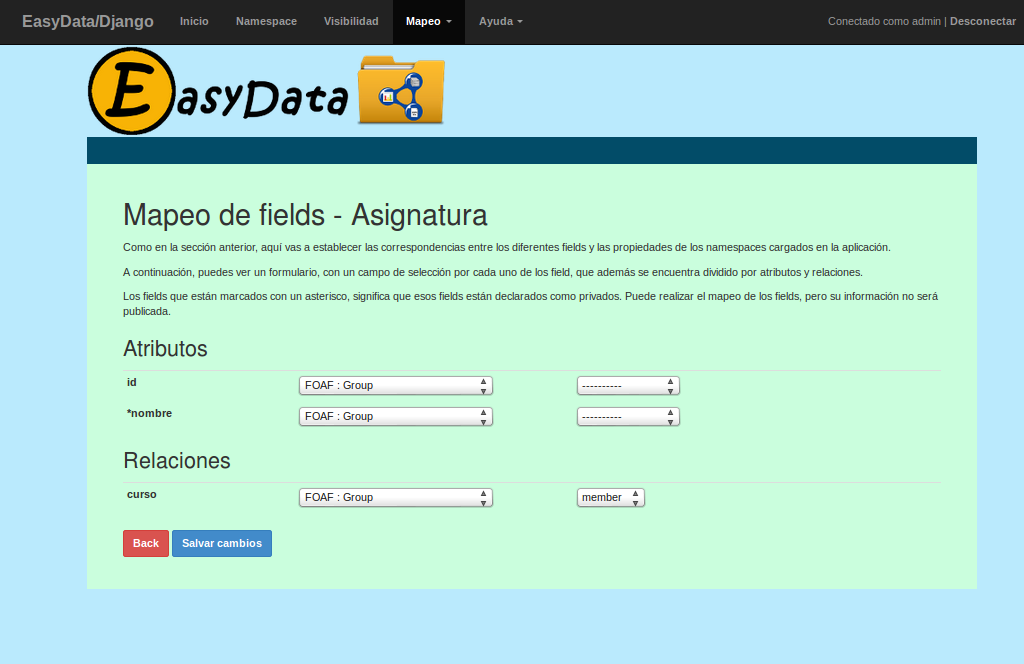
\includegraphics[width=1\textwidth]{manual_usuario/mapea_fields.png}
    \end{center}
    \caption{Pantalla de mapeo de los fields de un determinado modelo}
    \label{fig:mapea_fields}
\end{figure}

\subsection{Publicación de los datos}

Una vez llegados a este punto, donde ya tenemos cargados los namespaces que
vamos a utilizar, tenemos configurada la privacidad de nuestros datos y el mapeo
de los mismos con los namespaces, solo queda publicar los datos de los mismos.

Para la publicación de los datos de los modelos de nuestro proyecto, existen
distintas posibilidades, según el formato y la vía a través de la cual
los queramos publicar:
\begin{itemize}
    \item A través de url generadas para instancias en concreto de los modelos,
    para todas las instancias de un modelos, o para todos los modelos mapeados
    con una determinada entidad de un namespace.
    \item Mediante código HTML, usando los formatos para el marcado de
    etiquetas HTML, como son RDFa y Microdata.
    \item A través de la plataforma D2Rq haciendo uso del endpoint SPARQL que
    ofrece.
\end{itemize}

\subsubsection{Mediante URLs}

Como hemos comentado anteriormente, una de las posibles formas que hay para
publicar los datos de su aplicación es a través del uso de URLs. Estas URLs
servirán sus datos en formatos como puede ser RDF/XML, RDF/Ntriples o
RDF/Trutle.

Para los ejemplos, supondremos que nuestro proyecto se encuentra instalado en la
URL 127.0.0.1:8000.

La aplicación EasyData/Django creará automáticamente tres tipos diferentes de
URLs:
\begin{itemize}
    \item URLs específicas para instancias concretas de cada uno de los modelos.
        Estas URLs están compuestas de la aplicación, el tipo (la entidad),
        modelo y clave primaria de la instancia, de la siguiente forma:
    \begin{center}
        \textit{http://127.0.0.1:8000/easydata/publish/instance/\textbf{aplicación}/\textbf{tipo}-\textbf{modelo}/\textbf{pk}.(xml|nt|ttl)}
    \end{center}
        Donde las palabras marcadas en negrita, se sustituirán por los datos
        comentados anteriormente, y la clave primaria irá seguida del formato en
        el que deseamos recibir los datos.
    \item También se crearán URLs concretas para cada modelo de nuestro
        proyecto, de tal forma que nos devolverá un fichero RDF con cada una de
        las instancias de dicho modelo. Dicha URL será de la siguiente forma:
    \begin{center}
        \textit{http://127.0.0.1:8000/easydata/publish/model/\textbf{aplicación}/\textbf{tipo}-\textbf{modelo}.(xml|nt|ttl)}
    \end{center}
        Donde las palabras marcadas en negrita, se sustituirán por los nombres
        de la aplicación y del modelo, seguido el modelo del formato en el que
        deseamos recibir los datos.
    \item Por último, también se crearán URLs concretas para cada una de las
        entidades de los namespaces, de tal forma que nos devolverá un fichero
        RDF con cada una de las instancias de los modelos mapeados con dicha
        entidad. Dicha URL tendrá el siguiente formato:
    \begin{center}
        \textit{http://127.0.0.1:8000/easydata/publish/type/\textbf{namesapace}/\textbf{entidad}.(xml|nt|ttl)}
    \end{center}
        Donde la palabra namespace, se sustituirá por el nombre del namespace y
        la palabra entidad por el nombre de la entidad de la que queremos
        obtener los datos en RDF, seguido del formato RDF en el que queremos que
        nos muestre los datos.
\end{itemize}

Para obtener información mucho mas concreta sobre todo lo comentado
anteriormente, puede consultar los apartados \textit{Modelos configurados} y
\textit{Entidades relacionadas} de la ayuda de la aplicación, donde se le
muestra todo lo comentado anteriormente, con ejemplos sobre datos reales de su
proyecto.

\subsubsection{Mediante RDFa y Microdata}

Para la inclusión de los datos en formato HTML en nuestras plantillas de Django,
se hará uso de los template tags de Django, que no son mas que funciones, que
pueden ejecutarse desde las plantillas.

Estos template tags, son funciones que reciben una determinada instancia de un
modelo, y generarán el html con las etiquetas RDFa o Microdata (siempre que el
modelo de la instancia haya sido mapeado previamente), de tal forma que cuando
una máquina acceda a nuestra aplicación, sea capaz de interpretar dichas marcas
como si de un fichero RDF se tratara y pueda interpretar la información de la
misma.

A continuación se indican los template tags disponibles, tanto para la
generación de código RDFa como Microdata.

\begin{center}
    \textbf{Microdata}
\end{center}

Para poder hacer uso de los template tags para la generación de código
Microdata, se deberá de cargar en la plantilla Django el módulo donde se
encuentran los template tags, incluyendo el siguiente código:

\begin{center}
    \textit{\{\% load easydata\_microdata \%\}}
\end{center}

Una vez tenemos cargados los template tags para microdata, únicamente tendremos
que hacer uso en las plantillas de ellos. Los template tags para microdata
disponibles son los siguientes:

En el caso de que queramos generar el código microdata de una determinada
instancia de un modelo y que muestre todos los fields visibles y mapeados de
este:
\begin{center}
    \textit{\{\% microdata\_ul instance \%\}}\\
    \textit{\{\% microdata\_div\_meta instance \%\}}\\
    \textit{\{\% microdata\_div\_span instance \%\}}\\
\end{center}

En el caso de que queramos generar el código microdata de una instancia,
indicándole el field en concreto que deseamos que muestre:
\begin{center}
    \textit{\{\% microdata\_li\_field instance ``field\_name'' \%\}}\\
    \textit{\{\% microdata\_meta\_field instance ``field\_name'' \%\}}\\
    \textit{\{\% microdata\_span\_field instance ``field\_name'' \%\}}\\
\end{center}

Cuando se hace uso de los templatetags que genera información de un determinado
field de la instancia, solo se genera la etiqueta HTML con el tipo del dato y el
dato en cuestión, por lo que no se incluye información del tipo de la instancia
a la que pertenece el dato, y que deberá incluir el usuario. Para ello, existe
un template tag de bloque que indicándole la instancia y el tipo de etiqueta que
queremos usar, nos genera dicha etiqueta de apertura y cierre HTML con la
información Microdata del tipo de la instancia. La estructura de este template
tag es la siguiente:
\begin{center}
    \textit{\{\% microdata\_open\_tag instance ``tag'' \%\}}\\
    Resto de etiquetas de la instancia\\
    \textit{\{\% microdata\_end\_tag \%\}}\\
\end{center}

A su vez, puede que una determinada instancia de un modelo de datos, contenga
relaciones con otra instancia de otro modelo, que por defecto al generar el
código HTML con Microdata, lo que se hará será generar una etiqueta con la
referencia a la URI que representa a la instancia con la que se relaciona. Puede
que sea de interés para el usuario, que en vez de dicha referencia, se generen
determinados datos de la instancia indicando la relación de esta (anidar
instancias). Para ello, existe también un template tag de bloque similar al
anterior, donde se indican las instancias relacionadas, el nombre del field y la
etiqueta mediante la cual relacionarlos. La estructura de este template tag es
la siguiente:
\begin{center}
    \textit{\{\% microdata\_open\_tag\_interno instancia\_padre instancia ``field'' ``tag'' \%\}}\\
    Resto de etiquetas de la instancia\\
    \textit{\{\% microdata\_end\_tag\_interno \%\}}\\
\end{center}

\begin{center}
    \textbf{RDFa}
\end{center}

Para poder hacer uso de los template tags para la generación de código RDFa, se
deberá de cargar en la plantilla Django el módulo donde se encuentran los
template tags, incluyendo el siguiente código:

\begin{center}
    \textit{\{\% load easydata\_rdfa \%\}}
\end{center}

Una vez tenemos cargados los template tags para RDFa, únicamente tendremos que
hacer uso en las plantillas de ellos. Los template tags para RDFa disponibles
son los siguientes:

En el caso de que queramos generar el código RDFa con una instancia y que
muestre todos los fields visibles y mapeados de este:
\begin{center}
    \textit{\{\% rdfa\_ul instance \%\}}\\
    \textit{\{\% rdfa\_div instance \%\}}\\
    \textit{\{\% rdfa\_div\_span instance \%\}}\\
\end{center}

En el caso de que queramos generar el código RDFa con instancias e
indicándole el field en concreto que deseamos que muestre:
\begin{center}
    \textit{\{\% rdfa\_li\_field instance ``field\_name'' \%\}}\\
    \textit{\{\% rdfa\_div\_field instance ``field\_name'' \%\}}\\
    \textit{\{\% rdfa\_span\_field instance ``field\_name'' \%\}}\\
\end{center}

Cuando se hace uso de los templatetags que genera información de un determinado
field de la instancia, solo se genera la etiqueta HTML con el tipo del dato y el
dato en cuestión, por lo que no se incluye información del tipo de la instancia
a la que pertenece el dato, y que deberá incluir el usuario. Para ello, existe
un template tag de bloque que indicándole la instancia y el tipo de etiqueta que
queremos usar, nos genera dicha etiqueta de apertura y cierre HTML con la
información RDFa del tipo de la instancia. La estructura de este template tag es
la siguiente:
\begin{center}
    \textit{\{\% rdfa\_open\_tag instance ``tag'' \%\}}\\
    Resto de etiquetas de la instancia\\
    \textit{\{\% rdfa\_end\_tag \%\}}\\
\end{center}

A su vez, puede que una determinada instancia de un modelo de datos, contenga
relaciones con otra instancia de otro modelo, que por defecto al generar el
código HTML con RDFa, lo que se hará será generar una etiqueta con la
referencia a la URI que representa a la instancia con la que se relaciona. Puede
que sea de interés para el usuario, que en vez de dicha referencia, se generen
determinados datos de la instancia indicando la relación de esta (anidar
instancias). Para ello, existe también un template tag de bloque similar al
anterior, donde se indican las instancias relacionadas, el nombre del field y la
etiqueta mediante la cual relacionarlos. La estructura de este template tag es
la siguiente:
\begin{center}
    \textit{\{\% rdfa\_open\_tag\_interno instancia\_padre instancia ``field'' ``tag'' \%\}}\\
    Resto de etiquetas de la instancia\\
    \textit{\{\% rdfa\_end\_tag\_interno \%\}}\\
\end{center}

Para obtener información más detallada sobre el uso de los template tags, puede
dirigirse al apartado de \textit{Uso en plantillas} de la ayuda de la
aplicación, donde podrá observar todos los template tags disponibles, así como
ejemplos de uso de cada uno y resultado generado, sobre datos reales de sus
modelos.

\subsubsection{Enlace en HTML}

Además de los template tags comentados anteriormente, dispone de un template tag
más, el cual a partir de una instancia de un modelo, genera el código HTML de un
enlace ``<a>'' con la URI donde se encuentra la información RDF de la instancia
que se le indicó.

Para hacer uso de este template tag, debe de importarlo de la siguiente forma:

\begin{center}
    \textit{\{\% load easydata\_links \%\}}
\end{center}

Y por último, el template tag se usará dentro de la plantilla Django de la
siguiente forma:

\begin{center}
    \textit{\{\% easydata\_include\_link instance \%\}}
\end{center}


\subsection{Generación de fichero D2Rq}

La plataforma D2RQ de código abierto, es un sistema para el acceso a los datos
de bases de datos relacionales, como si se tratasen de grafos RDF virtuales de
solo lectura. De esta forma, ofrece a los usuario acceso mediante RDF al
contenido relacional de las bases de datos, sin la necesidad de tener que
replicar estos sobre un almacenamiento en formato RDF. Resumiendo, haciendo uso
de D2RQ podrás:
\begin{itemize}
    \item Hacer consultas sobre una base de datos que no sea de tipo RDF
        haciendo uso de SPARQL.
    \item Acceder al contenido de la base de datos, como Linked Data sobre la
        web.
    \item Crear volcados personalizados de la base de datos en formato RDF.
    \item Acceder a información de una base de datos que no sea de tipo RDF,
        haciendo uso de la API Apache Jena.
\end{itemize}

Para realizar las tareas anteriormente citadas, el software D2Rq necesita de un
fichero de configuración, donde se plasme el mapeo entre las tablas y columnas
de la base de datos y las etiquetas de los distintos namespaces, de forma que
este software pueda procesar las consultas SPARQL y crear el contenido RDF. Este
fichero, puede ser generado en la aplicación EasyData/Django, haciendo uso del
mapeo realizado en la propia aplicación.

Para realizar dicho mapeo, al igual que cuando realizó la resolución de los
modelos y fields del proyecto, deberá ejecutar desde la terminal el siguiente
comando del manage.py de Django.

\begin{lstlisting}[frame=L, language=bash, basicstyle=\footnotesize]
$> python manage.py easydata_d2rq
\end{lstlisting}

Este comando le mostrará por pantalla la configuración en formato
\textit{Turtle} (ttl) realizada por usted en la aplicación lista para ser usada
en la aplicación D2Rq. Si desea guardar la configuración en un fichero, solo
tiene que redirigir la salida hacia un fichero de la siguiente forma:

\begin{lstlisting}[frame=L, language=bash, basicstyle=\footnotesize]
$> python manage.py easydata_d2rq > configuracion.ttl
\end{lstlisting}

Una vez generado el fichero, deberá editarlo mediante cualquier editor
compatible con este formato de fichero, para introducir las opciones de conexión
a la base de datos (nombre de usuario, contraseña, host, controlador, etc...).
Además, este se trata de un documento base con la estructura que hay definida de
la base de datos dentro de la aplicación, el cual usted podrá editar para añadir
nuevos tipos de relaciones, propiedades, etc...

Tenga en cuenta que el software D2Rq es bastante complejo y ofrece al usuario
una gran cantidad de posibilidades a la hora de trabajar con los datos y
realizar el mapeo de los mismo. Además, este software trabaja directamente sobre
la estructura de la base de datos y esta en los proyectos Django se encuentra
estructurada en función de la forma de trabajar del ORM del framework, de tal
forma que no siempre se corresponderán los modelos con las tablas existentes en
la base de datos, principalmente cuando existan herencias y relaciones
complejas. Por estas dos razones, el resultado final del fichero puede no ser
definitivo, sino que servirá como base para que el usuario no tenga que trabajar
desde un fichero completamente en blanco y pueda aprovechar gran parte del
trabajo realizado sobre la aplicación, pero este requerirá finalmente de la
intervención del usuario.

Finalmente, una vez tenga el fichero de configuración para D2Rq podrá realizar
multitud de acciones, como desplegar un servidor donde los usuarios puedan
consultar los datos publicados. Este servidor podrá ser desplegado directamente
desde la línea de comandos (\url{http://d2rq.org/d2r-server#command-line}), o
bien como una aplicación web J2EE dentro de un servidor Apache Tomcat o Jetty
(\url{http://d2rq.org/d2r-server#servlet-container}).

Para más información acerca de cómo realizar consultas, modificar los ficheros
de configuración D2Rq, ejecución del servidor web, y el resto de utilidades y
herramientas que le proporciona la plataforma D2Rq, consulte la página oficial
\cite{d2rq} donde se le explica todo esto mucho más detallado.

\subsection{Generación de gráfico}

A la vez que vaya realizando el mapeo de sus modelos y fields con las
correspondientes entidades y propiedades de los namespaces, podrá obtener un
grafo donde podrá visualizar dicha configuración. En ella se apreciarán cada uno
de los modelos con sus atributos, así como las relaciones existentes entre
modelos, y junto a cada uno de ellos, las entidades o propiedades de los
namespaces con las que están mapeados.

Para generar dicho grafo, deberá de hacer click sobre el apartado de
\textit{Mapeo}, y en el menú desplegable que le aparece, pulsar sobre la opción
de \textit{Generar grafo}. Automáticamente, la aplicación le devolverá un
fichero .png con el grafo indicado.

En caso de que el sistema no disponga de la aplicación GraphViz para la
generación de la imagen png, se le devolverá un fichero en formato .dot, a
partir del cual, podrá generar la imagen haciendo uso de la aplicación graphviz.
Para generar la imagen desde la interfaz gráfica de la aplicación graphviz, o
desde una terminal de escritorio, donde tendrá que ejecutar el siguiente
comando:

\begin{lstlisting}[frame=L, language=bash, basicstyle=\footnotesize]
$> dot grafo.dot -Tpng -o nombre_grafo.png
\end{lstlisting}

% TODO: cuando sepa exactamente si se incluirá esta parte

% Descripción del área de trabajo del sistema y las instrucciones concretas para hacer uso de las funcionalidades del sistema.
